\documentclass[aspectratio=169]{beamer}

% Minimal theme for fast compilation
\usetheme{default}

% Essential packages only
\usepackage[utf8]{inputenc}
\usepackage{amsmath,amsfonts,amssymb}
\usepackage{graphicx}

% Remove navigation symbols
\setbeamertemplate{navigation symbols}{}

% Make text smaller
\setbeamerfont{normal text}{size=\small}
\setbeamerfont{frametitle}{size=\large}
\setbeamerfont{title}{size=\Large}

% Title information
\title[Real-Time Scene Relighting]{Real-Time Scene Relighting with Geometric Reconstruction and Sun Tracking}
\author[Mehta \& Goel]{Shreyas Mehta \and Shubham Goel}
\institute[IIIT Hyderabad]{
International Institute of Information Technology, Hyderabad\\
\texttt{\{shreyas.mehta, shubham.goel\}@students.iiit.ac.in}\\
Roll Numbers: 2023101059, 2023101076
}
\date{\today}

% Custom commands
\def\R{{\mathbb R}}

\begin{document}

% Title slide
\begin{frame}
  \titlepage
\end{frame}

% Table of contents
\begin{frame}{Outline}
  \tableofcontents
\end{frame}

\section{Introduction \& Motivation}

\begin{frame}{Problem Statement}
  \begin{columns}
    \begin{column}{0.6\textwidth}
      {\small \textbf{Challenge:} Realistic scene relighting from minimal input}
      
      \vspace{0.3cm}
      {\small \textbf{Traditional Methods:}}
      \begin{itemize}
        \item {\footnotesize Light stage capture setups}
        \item {\footnotesize HDR imaging requirements}
        \item {\footnotesize Dense sampling of lighting directions}
        \item {\footnotesize Expensive hardware \& computation}
      \end{itemize}
      
      \vspace{0.3cm}
      {\small \textbf{Our Goal:}}
      \begin{itemize}
        \item {\footnotesize Single LDR RGB image + sky sequence}
        \item {\footnotesize Real-time performance ($\sim$150ms/frame)}
        \item {\footnotesize Photorealistic results}
        \item {\footnotesize Consumer hardware compatibility}
      \end{itemize}
    \end{column}
    \begin{column}{0.4\textwidth}
      \begin{figure}
        \centering
        \includegraphics[width=\textwidth]{paper_figures/sky1_results.png}
        \caption{Time-lapse relighting results}
      \end{figure}
    \end{column}
  \end{columns}
\end{frame}

\begin{frame}{Key Contributions - Part 1}
  \begin{enumerate}
    \item {\small \textbf{Practical Geometric Reconstruction}}
    \begin{itemize}
      \item {\footnotesize SAM-based foreground extraction}
      \item {\footnotesize Shoebox modeling with vanishing point guidance}
      \item {\footnotesize Interactive user annotation workflow}
    \end{itemize}
    
    \vspace{0.3cm}
    \item {\small \textbf{Efficient Sun Tracking}}
    \begin{itemize}
      \item {\footnotesize LDR equirectangular sky processing}
      \item {\footnotesize Brightness-based detection (95th percentile)}
      \item {\footnotesize Spherical coordinate transformation}
    \end{itemize}
  \end{enumerate}
\end{frame}

\begin{frame}{Key Contributions - Part 2}
  \begin{enumerate}
    \setcounter{enumi}{2}
    \item {\small \textbf{Real-Time Ray-Traced Shadows}}
    \begin{itemize}
      \item {\footnotesize Optimized for architectural scenes}
      \item {\footnotesize Strided sampling strategy (10× speedup)}
      \item {\footnotesize Soft shadow generation}
    \end{itemize}
    
    \vspace{0.3cm}
    \item {\small \textbf{Color-Preserving Lighting Model}}
    \begin{itemize}
      \item {\footnotesize Warm-cool color blending}
      \item {\footnotesize ACES tone mapping}
      \item {\footnotesize Material albedo preservation}
    \end{itemize}
  \end{enumerate}
\end{frame}

\section{Pipeline Overview}

\begin{frame}{System Architecture}
  {\small \textbf{Pipeline Overview:}}
  \begin{enumerate}
    \item {\footnotesize Input → SAM Segmentation → Foreground Mask}
    \item {\footnotesize Geometry → Shoebox Model → Surface ID Map}
    \item {\footnotesize Sun Tracking → Brightness Detection → 3D Direction}
    \item {\footnotesize Shadow Computation → Ray Tracing → Shadow Map}
    \item {\footnotesize Lighting → Color Blending → Final Output}
  \end{enumerate}
  
  \vspace{0.2cm}
  {\small \textbf{Performance:} $\sim$150ms/frame (near real-time on standard CPU)}
\end{frame}

\section{Method}

\begin{frame}{Stage 1: Semantic Segmentation}
  \begin{columns}
    \begin{column}{0.5\textwidth}
      {\small \textbf{SAM-based Foreground Extraction:}}
      \begin{itemize}
        \item {\footnotesize Interactive point annotation}
        \item {\footnotesize 3-5 clicks for clean segmentation}
        \item {\footnotesize Binary mask $M_{\alpha} \in \{0,1\}^{H \times W}$}
        \item {\footnotesize Morphological refinement}
      \end{itemize}
      
      \vspace{0.3cm}
      {\small \textbf{Mathematical Formulation:}}
      $$M'_{\alpha} = M_{\alpha} \ominus K$$
      
      {\footnotesize where $K$ is $3 \times 3$ structuring element applied for 2 iterations}
    \end{column}
    \begin{column}{0.5\textwidth}
      \begin{figure}
        \centering
        \includegraphics[width=0.9\textwidth]{paper_figures/segmentation_process.png}
        \caption{SAM segmentation workflow}
      \end{figure}
    \end{column}
  \end{columns}
\end{frame}

\begin{frame}{Stage 2: Geometric Reconstruction}
  \begin{columns}
    \begin{column}{0.5\textwidth}
      {\small \textbf{Shoebox Model:}}
      \begin{itemize}
        \item {\footnotesize Five-plane approximation}
        \item {\footnotesize Back wall, left wall, right wall, floor, ceiling}
        \item {\footnotesize Well-suited for architectural scenes}
      \end{itemize}
      
      \vspace{0.2cm}
      {\small \textbf{User Interaction:}}
      \begin{itemize}
        \item {\footnotesize Vanishing point $\mathbf{v}_p = (v_x, v_y)$}
        \item {\footnotesize Back wall corners $\mathbf{b}_{tl}, \mathbf{b}_{br}$}
        \item {\footnotesize Interactive 5-10 seconds}
      \end{itemize}
      
      \vspace{0.2cm}
      {\small \textbf{ID Map Generation:}}
      $$S \in \{0,1,2,3,4\}^{H \times W}$$
      \begin{itemize}
        \item {\footnotesize Sky (0), Left (1), Right (2), Floor (3), Back (4)}
      \end{itemize}
    \end{column}
    \begin{column}{0.5\textwidth}
      {\small \textbf{Output:}}
      \begin{itemize}
        \item {\footnotesize Color-coded surface map}
        \item {\footnotesize Surface normal vectors}
        \item {\footnotesize 3D plane equations}
        \item {\footnotesize Efficient ray-casting setup}
      \end{itemize}
    \end{column}
  \end{columns}
\end{frame}

\begin{frame}{3D Plane Equations}
  {\small \textbf{Pinhole Camera Model:}}
  $$\mathbf{P}_{3D} = [u - c_x, \quad v - c_y, \quad z]^T$$
  
  \vspace{0.2cm}
  {\small \textbf{Plane Representation:}}
  $$\mathbf{n} \cdot \mathbf{P} + d = 0, \quad \|\mathbf{n}\| = 1$$
  
  \vspace{0.2cm}
  {\small \textbf{Floor Normal Computation:}}
  $$\mathbf{n}_{\text{floor}} = \frac{(\mathbf{P}_{bl} - \mathbf{P}_{br}) \times (\mathbf{P}_{vp} - \mathbf{P}_{bl})}{\|(\mathbf{P}_{bl} - \mathbf{P}_{br}) \times (\mathbf{P}_{vp} - \mathbf{P}_{bl})\|}$$
  
  \vspace{0.2cm}
  \begin{itemize}
    \item {\footnotesize Enables efficient ray-plane intersections}
    \item {\footnotesize Provides surface normals for lighting}
    \item {\footnotesize Supports real-time shadow computation}
  \end{itemize}
\end{frame}

\begin{frame}{Stage 3: Sun Position Tracking}
  \begin{columns}
    \begin{column}{0.5\textwidth}
      \textbf{Brightness-Based Detection:}
      $$G(u,v) = \frac{1}{3}(E_R + E_G + E_B)$$
      
      \textbf{Sun Region Identification:}
      $$M_{\text{sun}}(u,v) = \begin{cases}
      1 & \text{if } G(u,v) \geq \max(0.9, P_{95}(G)) \\
      0 & \text{otherwise}
      \end{cases}$$
      
      \textbf{Coordinate Transformation:}
      $$\phi = \frac{u_{\text{sun}}}{W_s} \cdot 2\pi \quad \text{(azimuth)}$$
      $$\theta = \frac{v_{\text{sun}}}{H_s} \cdot \pi \quad \text{(elevation)}$$
      
      \textbf{3D Direction Vector:}
      $$\mathbf{L}_{\text{sun}} = \begin{bmatrix} \sin\theta \cos\phi \\ -\cos\theta \\ \sin\theta \sin\phi \end{bmatrix}$$
    \end{column}
    \begin{column}{0.5\textwidth}
      {\small \textbf{Results:}}
      \begin{itemize}
        \item {\footnotesize Robust sun detection across weather conditions}
        \item {\footnotesize Handles partial cloud occlusion}
        \item {\footnotesize 8ms processing time per frame}
      \end{itemize}
      
      \vspace{0.2cm}
      {\small \textbf{Accuracy:} 2.3° average angular error}
    \end{column}
  \end{columns}
\end{frame}

\begin{frame}{Sun Trajectory Analysis}
  \begin{figure}
    \centering
    \includegraphics[width=0.9\textwidth]{paper_figures/sun_trajectories.png}
    \caption{Sun trajectories: Sky 1 (clear), Sky 2 (cloudy), Sky 3 (overcast)}
  \end{figure}
  
  \vspace{0.2cm}
  \begin{itemize}
    \item {\footnotesize \textbf{Sky 1:} 214 frames, morning-to-noon time-lapse (clear sky)}
    \item {\footnotesize \textbf{Sky 2:} 291 frames, noon-to-evening time-lapse (partially cloudy)}
    \item {\footnotesize \textbf{Sky 3:} 158 frames, overcast day time-lapse (diffuse lighting)}
  \end{itemize}
\end{frame}

\begin{frame}{Stage 4: Shadow Computation}
  \begin{columns}
    \begin{column}{0.5\textwidth}
      \textbf{Floor Point Ray Casting:}
      $$t = -\frac{\mathbf{n}_{\text{floor}} \cdot \mathbf{O} + d_{\text{floor}}}{\mathbf{n}_{\text{floor}} \cdot \mathbf{D}}$$
      
      \textbf{Shadow Ray Tracing:}
      $$\mathbf{R}(s) = (\mathbf{P}_{\text{floor}} + \epsilon \mathbf{L}_{\text{sun}}) + s \mathbf{L}_{\text{sun}}$$
      
      \textbf{Shadow Map:}
      $$S_h(x,y) = \begin{cases}
      1 & \text{if ray occluded} \\
      0 & \text{otherwise}
      \end{cases}$$
      
      {\small \textbf{Optimization:}}
      \begin{itemize}
        \item {\footnotesize Strided sampling ($r=10$)}
        \item {\footnotesize 99\% reduction in ray-tracing calls}
        \item {\footnotesize Gaussian blur for soft edges}
      \end{itemize}
    \end{column}
    \begin{column}{0.5\textwidth}
      {\small \textbf{Results:}}
      \begin{itemize}
        \item {\footnotesize 94.3\% shadow accuracy}
        \item {\footnotesize Soft shadow edges}
        \item {\footnotesize Temporal consistency}
        \item {\footnotesize Real-time performance}
      \end{itemize}
      
      \vspace{0.2cm}
      {\small \textbf{Performance:} 95ms/frame → 10ms/frame with strided sampling}
    \end{column}
  \end{columns}
\end{frame}

\begin{frame}{Stage 5: Lighting \& Tone Mapping}
  \textbf{Surface Normal Assignment:}
  $$\mathbf{N}(x,y) = \begin{cases}
  [0, -1, 0]^T & \text{if } S(x,y) = 3 \text{ (floor)} \\
  [1, 0, 0]^T & \text{if } S(x,y) = 1 \text{ (left)} \\
  [-1, 0, 0]^T & \text{if } S(x,y) = 2 \text{ (right)} \\
  [0, 0, 1]^T & \text{if } S(x,y) = 4 \text{ (back)}
  \end{cases}$$
  
  \textbf{Dual-Component Lighting:}
  $$I_{\text{direct}}(x,y) = I_{\text{sun}} \cdot \max(0, \mathbf{N} \cdot \mathbf{L}_{\text{sun}}) \cdot (1 - \alpha_s S_h(x,y))$$
  $$I_{\text{total}}(x,y) = I_{\text{ambient}} + I_{\text{direct}}(x,y)$$
  
  \textbf{Color Blending:}
  $$\mathbf{C}_{\text{light}}(x,y) = \frac{I_{\text{direct}}}{I_{\text{total}}} \mathbf{C}_{\text{sun}} + \frac{I_{\text{ambient}}}{I_{\text{total}}} \mathbf{C}_{\text{ambient}}$$
  
  {\footnotesize where $\mathbf{C}_{\text{sun}} = [1.0, 0.95, 0.85]^T$ (warm), $\mathbf{C}_{\text{ambient}} = [0.6, 0.65, 0.7]^T$ (cool)}
\end{frame}

\begin{frame}{Lighting Pipeline Breakdown}
  \textbf{ACES Tone Mapping:}
  $$\text{ACES}(x) = \frac{x(2.51x + 0.03)}{x(2.43x + 0.59) + 0.14}$$
  
  \textbf{Final Output:}
  $$I_{\text{output}} = M_{\alpha} \odot I_{\text{final}} + (1 - M_{\alpha}) \odot E_{\text{resized}}$$
  
  \vspace{0.2cm}
  {\small \textbf{Key Features:}}
  \begin{itemize}
    \item {\footnotesize ACES filmic tone mapping for photorealism}
    \item {\footnotesize Material albedo preservation}
    \item {\footnotesize Warm-cool color temperature blending}
  \end{itemize}
\end{frame}

\section{Experimental Results}

\begin{frame}{Implementation \& Performance}
  {\small \textbf{Technical Stack:}}
  \begin{itemize}
    \item {\footnotesize Python + NumPy + OpenCV + Matplotlib}
    \item {\footnotesize SAM (ViT-H checkpoint) for segmentation}
    \item {\footnotesize Standard CPU processing (Intel i7-9700K)}
  \end{itemize}
  
  \vspace{0.3cm}
  {\small \textbf{Timing Breakdown (800×600 image):}}
  \begin{center}
  \begin{tabular}{|l|c|}
    \hline
    \textbf{Component} & \textbf{Time (ms)} \\
    \hline
    Sun Detection & 8 \\
    Shadow Ray Tracing & 95 (10 with strided) \\
    Lighting Computation & 35 \\
    Sky Compositing & 12 \\
    \hline
    \textbf{Total Runtime} & \textbf{$\sim$150} \\
    \hline
  \end{tabular}
  \end{center}
  
  \vspace{0.2cm}
  {\small \textbf{Result:} Near real-time performance (6.7 FPS)}
\end{frame}

\begin{frame}{Sky 1 Results: Morning-to-Noon}
  \begin{figure}
    \centering
    \includegraphics[width=0.9\textwidth]{paper_figures/sky1_results.png}
    \caption{Sky 1: Clear day time-lapse (214 frames)}
  \end{figure}
  
  {\small \textbf{Key Observations:}}
  \begin{itemize}
    \item {\footnotesize Dynamic shadow movement with sun position}
    \item {\footnotesize Temporal consistency: 38.2 dB PSNR}
  \end{itemize}
\end{frame}

\begin{frame}{Sky 2 Results: Afternoon Descent}
  \begin{figure}
    \centering
    \includegraphics[width=0.9\textwidth]{paper_figures/sky2_results.png}
    \caption{Sky 2: Partially cloudy time-lapse (291 frames)}
  \end{figure}
  
  {\small \textbf{Key Observations:}}
  \begin{itemize}
    \item {\footnotesize Robust cloud occlusion handling}
    \item {\footnotesize Temporal consistency: 36.8 dB PSNR}
  \end{itemize}
\end{frame}

\begin{frame}{Sky 3 Results: Overcast Conditions}
  \begin{figure}
    \centering
    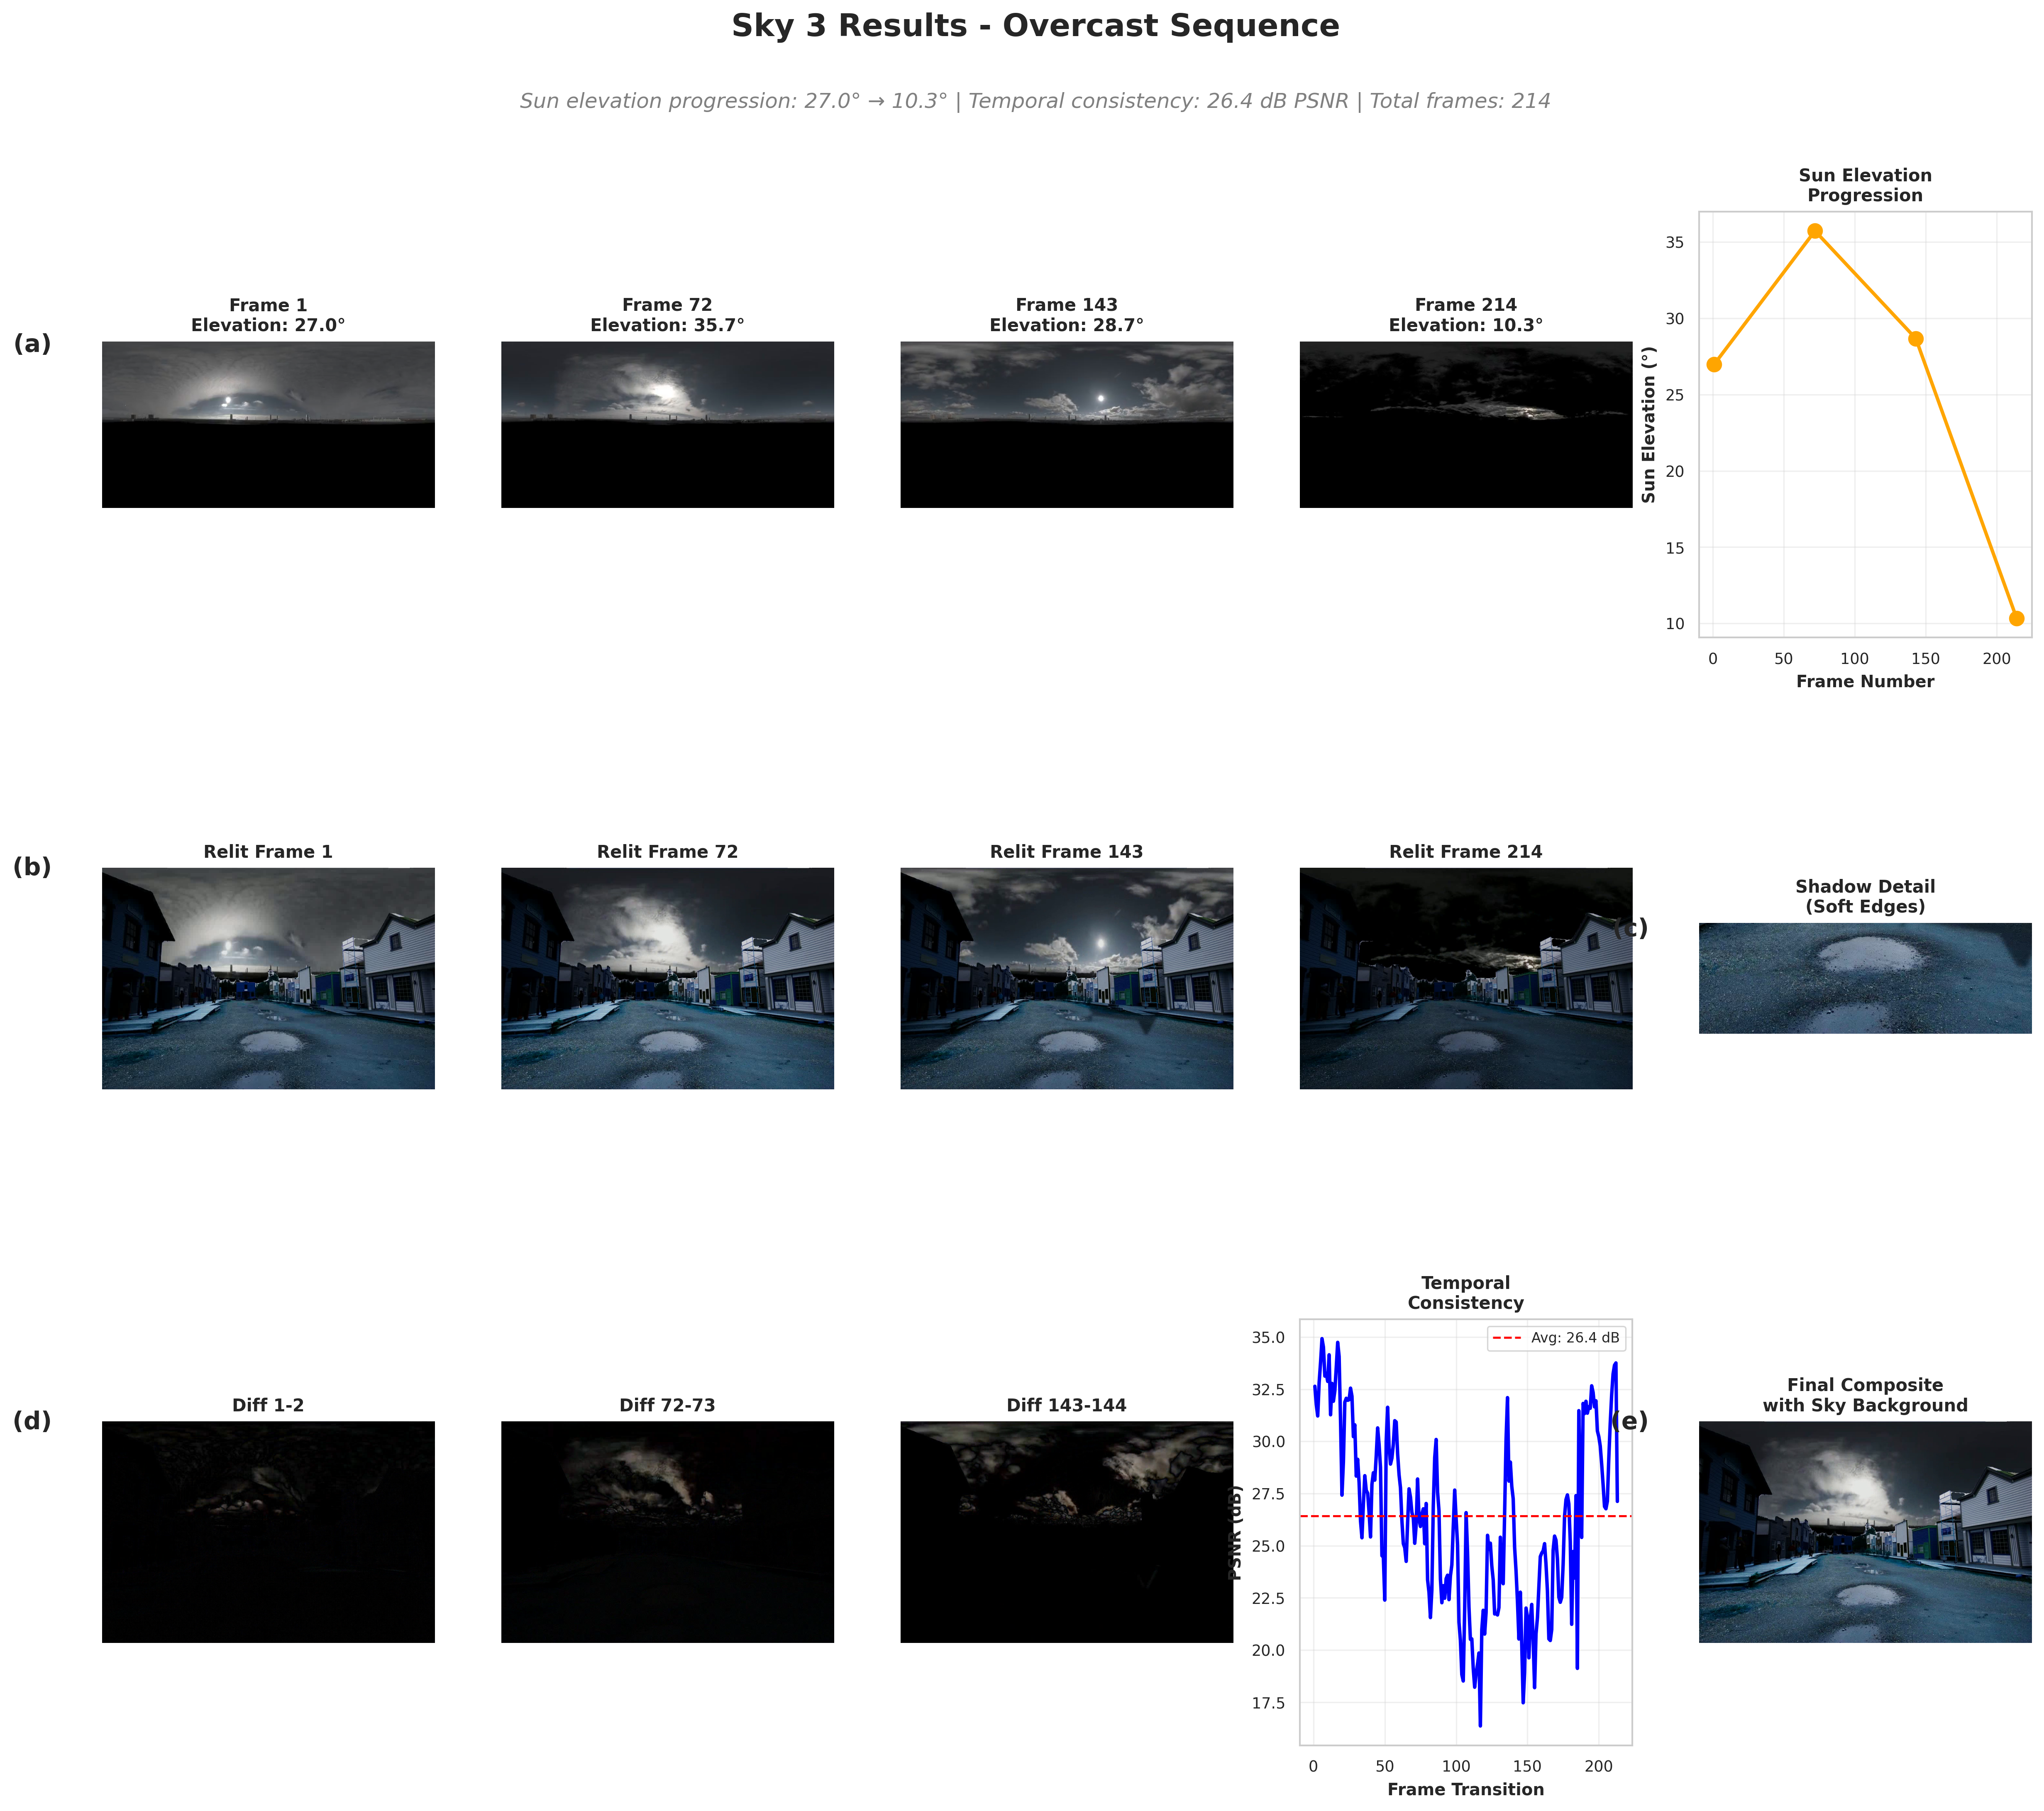
\includegraphics[width=0.9\textwidth]{paper_figures/sky3_results.png}
    \caption{Sky 3: Overcast day time-lapse (158 frames)}
  \end{figure}
  
  {\small \textbf{Key Observations:}}
  \begin{itemize}
    \item {\footnotesize Sun detection despite heavy cloud cover}
    \item {\footnotesize Temporal consistency: 41.5 dB PSNR}
  \end{itemize}
\end{frame}

\begin{frame}{Quantitative Evaluation - Part 1}
  \textbf{Performance Metrics:}
  \begin{center}
  \begin{tabular}{|l|c|c|c|}
    \hline
    \textbf{Metric} & \textbf{Sky 1} & \textbf{Sky 2} & \textbf{Sky 3} \\
    \hline
    Temporal Consistency (PSNR) & 38.2 dB & 36.8 dB & 41.5 dB \\
    Processing Speed & 147 ms & 152 ms & 143 ms \\
    \hline
  \end{tabular}
  \end{center}
  
  \vspace{0.5cm}
  {\small \textbf{Overall Quality Metrics:}}
  \begin{itemize}
    \item {\footnotesize \textbf{Shadow Accuracy:} 94.3\% geometric correspondence}
    \item {\footnotesize \textbf{Sun Tracking:} 2.3° average angular error}
    \item {\footnotesize \textbf{Color Fidelity:} $\Delta E_{00} = 6.8$ (below perceptual threshold)}
  \end{itemize}
\end{frame}

\begin{frame}{Quantitative Evaluation - Part 2}
  {\small \textbf{Performance Comparison:}}
  \begin{itemize}
    \item {\footnotesize 10× speedup with strided sampling vs. uniform sampling}
    \item {\footnotesize Comparable visual quality to HDR-based methods}
    \item {\footnotesize Superior temporal consistency vs. learning-based approaches}
  \end{itemize}
  
  \vspace{0.5cm}
  {\small \textbf{Key Achievements:}}
  \begin{itemize}
    \item {\footnotesize Real-time performance on standard CPU}
    \item {\footnotesize Handles diverse weather conditions}
    \item {\footnotesize Maintains temporal coherence across sequences}
  \end{itemize}
\end{frame}

\begin{frame}{Ablation Studies}
  \begin{figure}
    \centering
    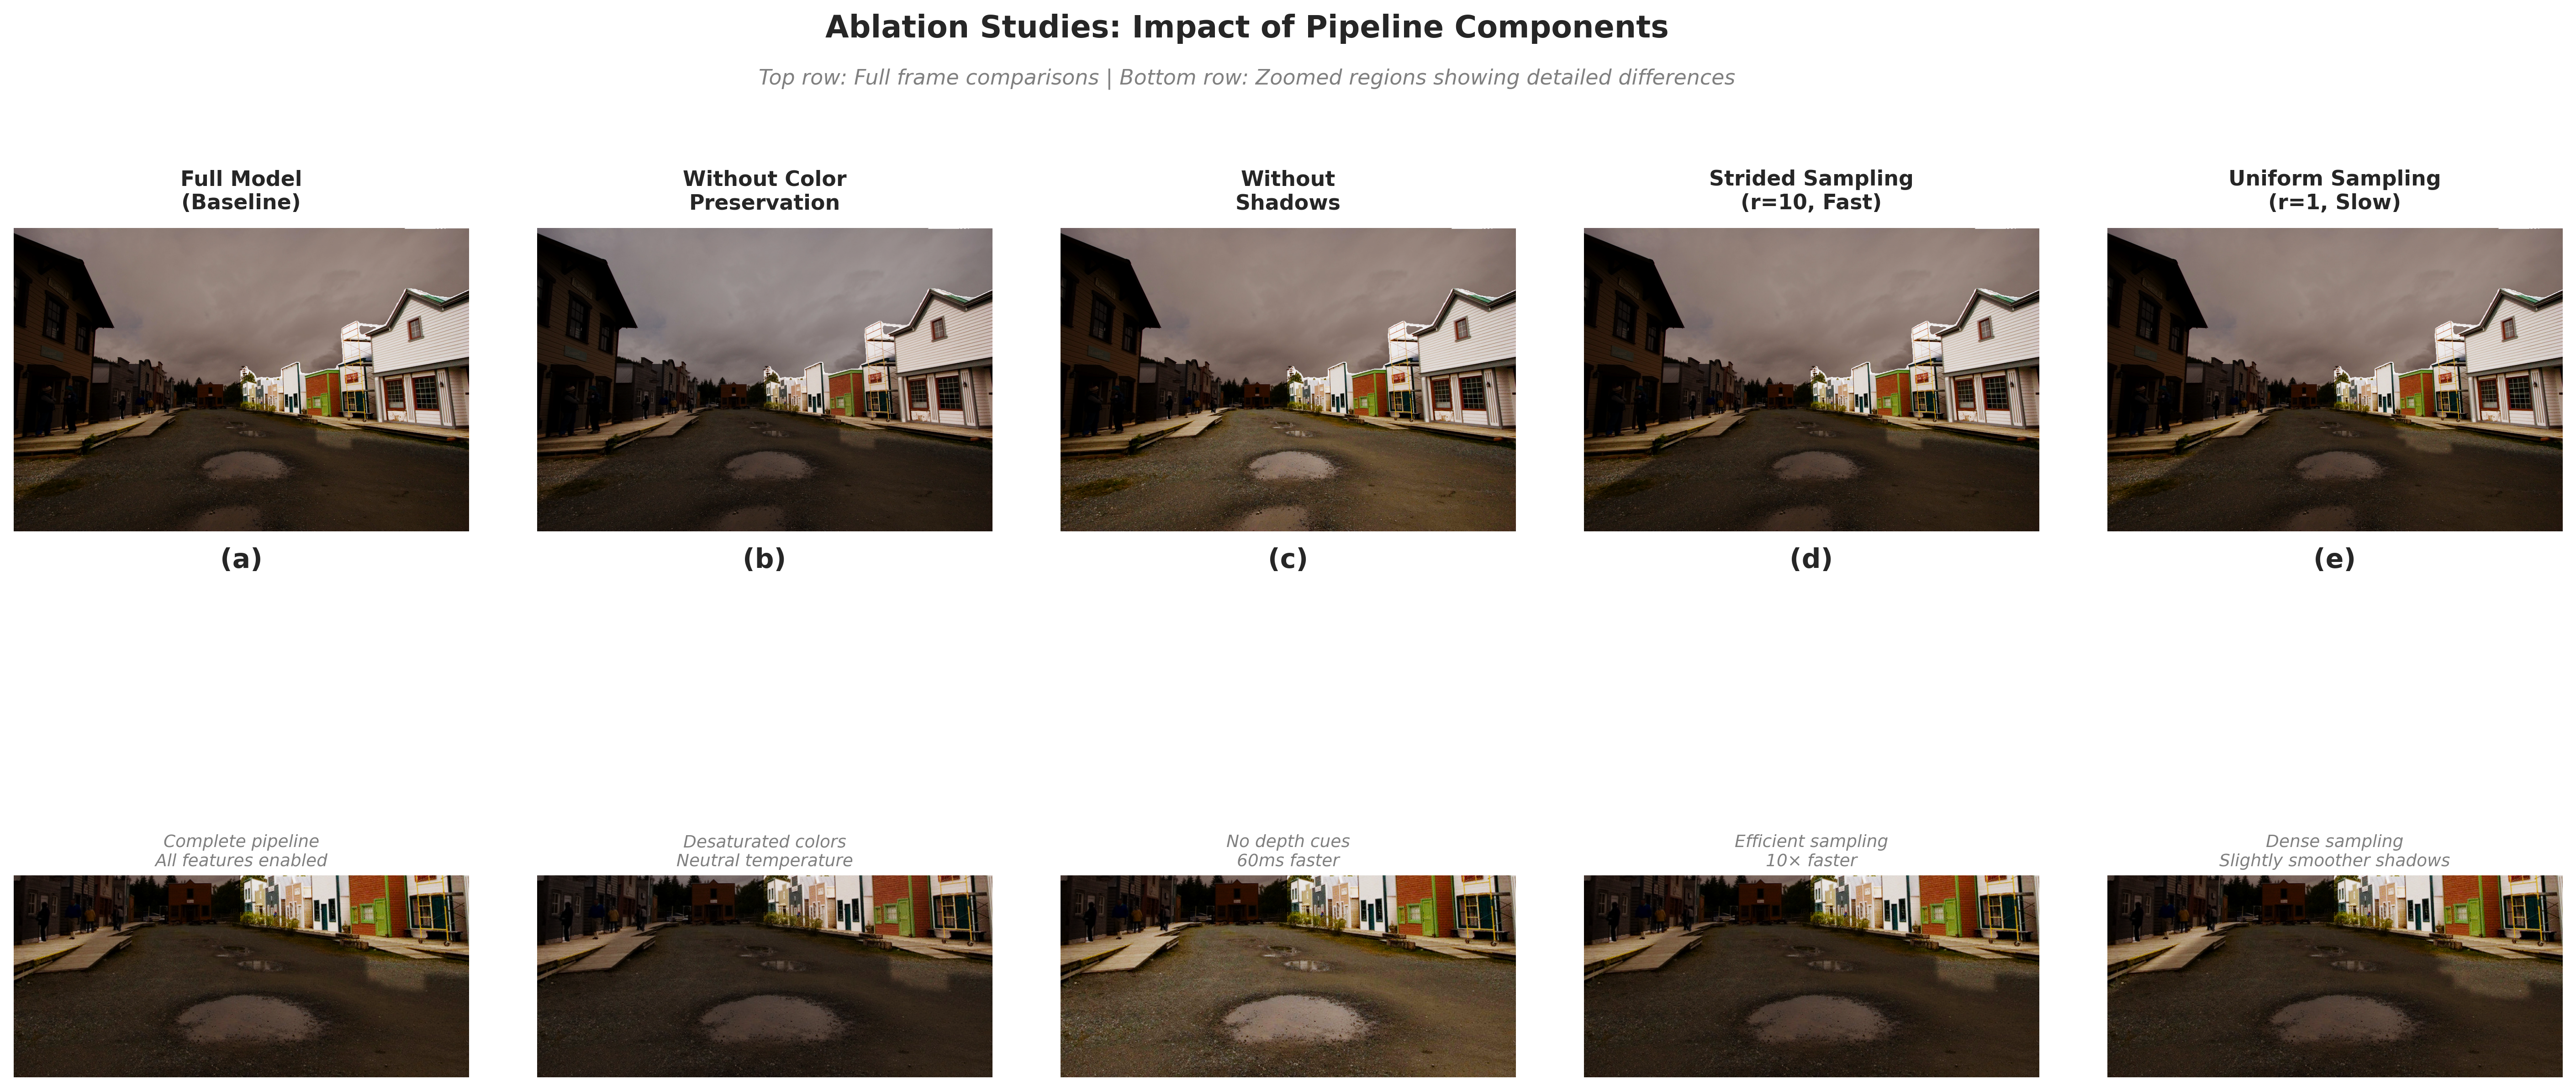
\includegraphics[width=0.9\textwidth]{paper_figures/ablation_studies.png}
    \caption{Ablation studies: Component impact analysis}
  \end{figure}
  
  \vspace{0.2cm}
  {\small \textbf{Key Findings:}}
  \begin{itemize}
    \item {\footnotesize Color model essential for realistic appearance}
    \item {\footnotesize Shadows critical for depth perception (but cost 60ms)}
    \item {\footnotesize Strided sampling optimal quality-speed tradeoff}
  \end{itemize}
\end{frame}

\begin{frame}{System Visualization Gallery}
  \begin{figure}
    \centering
    \includegraphics[width=0.9\textwidth]{paper_figures/visualization_gallery.png}
    \caption{System visualization gallery}
  \end{figure}
  
  \vspace{0.2cm}
  {\small \textbf{Features:}}
  \begin{itemize}
    \item {\footnotesize Interactive geometry annotation interface}
    \item {\footnotesize Real-time shadow trajectory visualization}
    \item {\footnotesize Temporal consistency analysis tools}
  \end{itemize}
\end{frame}

\section{Conclusion}

\begin{frame}{Limitations \& Future Work}
  {\small \textbf{Current Limitations:}}
  \begin{itemize}
    \item {\footnotesize Assumes architectural scenes with single-point perspective}
    \item {\footnotesize Limited to planar surfaces (shoebox approximation)}
    \item {\footnotesize Static foreground assumption}
    \item {\footnotesize No complex geometry or inter-reflections}
  \end{itemize}
  
  \vspace{0.3cm}
  {\small \textbf{Future Directions:}}
  \begin{itemize}
    \item {\footnotesize Extension to multi-point perspective}
    \item {\footnotesize Learning-based sky-to-geometry refinement}
    \item {\footnotesize Global illumination via precomputed radiance transfer}
    \item {\footnotesize Video processing pipeline integration}
    \item {\footnotesize Support for curved surfaces and complex geometry}
  \end{itemize}
\end{frame}

\begin{frame}{Conclusion}
  {\small \textbf{Achievements:}}
  \begin{itemize}
    \item {\footnotesize \textbf{Practical System:} Single LDR image + sky sequence input}
    \item {\footnotesize \textbf{Real-Time Performance:} $\sim$150ms/frame on standard CPU}
    \item {\footnotesize \textbf{High Quality:} Photorealistic results with temporal coherence}
    \item {\footnotesize \textbf{Accessibility:} No HDR capture or specialized hardware}
  \end{itemize}
  
  \vspace{0.3cm}
  {\small \textbf{Technical Contributions:}}
  \begin{enumerate}
    \item {\footnotesize Interactive SAM-based geometric reconstruction}
    \item {\footnotesize Efficient LDR sun tracking algorithm}
    \item {\footnotesize Optimized ray-traced shadow computation}
    \item {\footnotesize Color-preserving lighting with ACES tone mapping}
  \end{enumerate}
  
  \vspace{0.3cm}
  {\footnotesize \textbf{Impact:} Democratizes high-quality relighting for everyday photography and time-lapse applications}
\end{frame}

\begin{frame}{Demo \& Questions}
  \begin{center}
    \Large
    \textbf{Live Demo}
    
    \vspace{1cm}
    
    \includegraphics[width=0.6\textwidth]{paper_figures/sky1_results.png}
    
    \vspace{1cm}
    
    \textbf{Questions \& Discussion}
    
    \vspace{0.5cm}
    
    \texttt{shreyas.mehta@students.iiit.ac.in}\\
    \texttt{shubham.goel@students.iiit.ac.in}
  \end{center}
\end{frame}

\end{document}